\documentclass[tikz,margin=0mm]{standalone}

\usepackage{amsmath}

\usetikzlibrary{arrows}
\usetikzlibrary{decorations.pathreplacing}
\usetikzlibrary{shadows,fadings}
\usetikzlibrary{shadows.blur}
\usetikzlibrary{fit}
\usetikzlibrary{calc}

\tikzset{geometry/.style=thick}
\tikzset{feederElectrode/.style={fill=black!30!white, draw=black!80!white}}
\tikzset{electrolyte/.style={fill=black!10!white, draw=black!80!white}}

\begin{document}
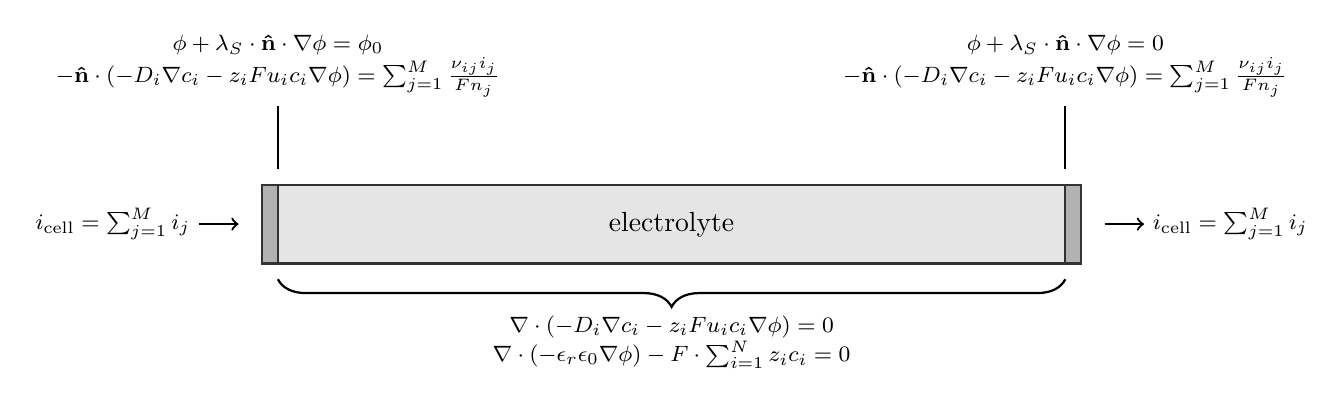
\begin{tikzpicture}[geometry]
\def \sternLayerWidth{0.8}
\fill[electrolyte,draw=none] (0,0) rectangle +(10,1) node[pos=0.5,anchor=center,align=center]{electrolyte};
\draw[electrolyte] (0,0) -- +(10,0) +(10,1) -- +(0,1);
\filldraw[feederElectrode] (-0.2,0) rectangle +(0.2,1);
\filldraw[feederElectrode] (10,0) rectangle +(0.2,1);
  
% electrode BC
\draw (0,2) node[node font=\footnotesize,anchor=south,align=center] {
  	$\phi + \lambda_S \cdot \mathbf{\hat{n}} \cdot \nabla \phi = \phi_0$\\
  	$-\mathbf{\hat{n}} \cdot ( -D_i \nabla c_i - z_i F u_i c_i \nabla \phi ) =  \sum_{j=1}^M \frac{\nu_{ij} i_j}{F n_j}$
	};
\draw (0,2) -- +(0,-0.8);
  
% bulk BC
\draw (10,2) node[node font=\footnotesize,anchor=south,align=center] {
  	$\phi + \lambda_S \cdot \mathbf{\hat{n}} \cdot \nabla \phi = 0$\\
  	$-\mathbf{\hat{n}} \cdot ( -D_i \nabla c_i - z_i F u_i c_i \nabla \phi ) =  \sum_{j=1}^M \frac{\nu_{ij} i_j}{F n_j}$
  	};
\draw (10,2) -- +(0,-0.8);
  
\draw[->] (-1,0.5) -- (-0.5,0.5) node[pos=0,anchor=east,node font=\footnotesize] {$i_\text{cell} = \sum_{j=1}^M i_j$};
\draw[->] (10.5,0.5) -- (11,0.5) node[anchor=west,node font=\footnotesize] {$i_\text{cell} = \sum_{j=1}^M i_j$};
  
%% governing eq
\draw [decorate,decoration={brace,amplitude=10pt},xshift=0,yshift=0] (10,-0.2) -- +(-10,0) node [node font=\footnotesize,anchor=north,midway,yshift=-10pt,align=center]  {$ \nabla \cdot ( -D_i \nabla c_i - z_i F u_i c_i \nabla \phi ) = 0 $ \\
  	$\nabla \cdot ( - \epsilon_r \epsilon_0 \nabla \phi ) - F \cdot \sum_{i=1}^N z_i c_i  = 0$ 
  	}; 
\end{tikzpicture}
\end{document}